\section{Auswertung}%
\label{sec:auswertung}
\subsection{Linearverst\"arker}
Die allgemeine, frequenzabhängige Verstärkung $V\!\left(\nu\right)$ wird gegen die Frequenz $\nu$ in einem doppellogarithmischen Diagramm aufgetragen.
Es wird ein Fit für den Verstärkungsfaktor für Tiefpässe berechnet, nach
Gleichung~\eqref{eq:tiefpass}:
\begin{equation}\label{eq:fit_tiefpass}
  V_\text{theo} = \frac{V'_{\text{exp}}}{\sqrt{1 + {\left({\frac{\nu}{\nu_\text{G}}}\right)}^{2}}}.
\end{equation}

Hierbei ist $V'_{\text{exp}}$ der gemessene Verstärkungsfaktor.
Die Messwerte der Verstärkungsfaktoren in Abhängigkeit der Frequenz
sind mit dem Fit in den Abbildungen~\ref{fig:lin_verst_01} bis~\ref{fig:lin_verst_04} dargestellt.
Die vier verschiedenen Konfigurationen der beiden Widerstände (vgl. Abbildung~\ref{fig:lin})
sind in den Abbildungsunterschriften zu finden,
die Grenzfrequenz $\nu_\text{G}$ und der Verstärkungsfaktor $V_\text{exp}$ in der entsprechenden Legende.

\begin{figure}[ht]
  \centering
  \includegraphics[width=\textwidth]{build/lin_verst_01__r1_200__rn_470__u1_100.pdf}
  \caption{Linearer Verstärker mit $R_1 = \SI{200}{\kilo\ohm}$, $R_N = \SI{470}{\kilo\ohm}$.}
  \label{fig:lin_verst_01}
\end{figure}

\begin{figure}[ht]
  \centering
  \includegraphics[width=\textwidth]{build/lin_verst_02__r1_200__rn_100__u1_100.pdf}
  \caption{Linearer Verst\"arker mit $R_1 = \SI{200}{\kilo\ohm}$, $R_N = \SI{100}{\kilo\ohm}$}
  \label{fig:lin_verst_02}
\end{figure}

\begin{figure}[ht]
  \centering
  \includegraphics[width=\textwidth]{build/lin_verst_03__r1_100__rn_470__u1_100.pdf}
  \caption{Linearer Verst\"arker mit $R_1 = \SI{100}{\kilo\ohm}$, $R_N = \SI{470}{\kilo\ohm}$}
  \label{fig:lin_verst_03}
\end{figure}

\begin{figure}[ht]
  \centering
  \includegraphics[width=\textwidth]{build/lin_verst_04__r1_470__rn_100__u1_100.pdf}
  \caption{Linearer Verst\"arker mit $R_1 = \SI{470}{\kilo\ohm}$, $R_N = \SI{100}{\kilo\ohm}$}
  \label{fig:lin_verst_04}
\end{figure}

Die Messergebnisse und theoretischen Werte der vier Konfigurationen der linearen Verstärker
sind in Tabelle~\ref{tab:vergleich} aufgetragen.
Hierbei ist $V_\text{exp}$ der Fitparameter aus Gleichung~\eqref{eq:fit_tiefpass}.
Gleichung~\eqref{eq:v_strich} wird nach dem Leerlaufverstärker $V$ umgestellt:
\begin{align}
  \frac{1}{V'} &= \frac{1}{V} + \frac{R_1}{R_N} \nonumber \\
  \Rightarrow \frac{1}{V} &= \frac{1}{V'} - \frac{R_1}{R_N} \nonumber \\
  \Rightarrow V &= \frac{1}{\frac{1}{V'} - \frac{R_1}{R_N}}
\end{align}
\begin{table}[ht]
  \centering
  \caption{Vergleich der Konfigurationen der linearen Verstärker.}
  \label{tab:vergleich}
  \begin{tabular}{
      S[table-format=1] |
      S[table-format=1.3]
      S[table-format=1.2\pm1.2,separate-uncertainty=true]
      S[table-format=2.3]
      S[table-format=2.1\pm1.1,separate-uncertainty=true]
      S[table-format=2.1]
      S[table-format=3.1]
  }
    \toprule
    {Nr.} & {$\sfrac{R_N}{R_1}$} & {$V_\text{exp}$} & {$\Delta V / \%$} & {$\nu_\text{G}
    / \si{\kilo\hertz}$} &  {$V'_\text{exp} \cdot \nu_\text{G} / \si{\kilo\hertz}$} & {$V$} \\
    \midrule
    1 & 2.35  & \num{2.2 \pm 0.01} & 6  & \num{1.7 \pm 1.4} & 3.8 & 39.2   \\
    2 & 0.5   & \num{0.2 \pm 0.01} & 51 & \num{2.4 \pm 0.5} & 0.6  & 0.5   \\
    3 & 4.7   & \num{4.6 \pm 0.04} & 1.2  & \num{0.9 \pm 0.4} & 4.3 & 374 \\
    4 & 0.213 & \num{0.05 \pm 0.01} & 77 & \num{4.3 \pm 0.1} & 0.2  & 0.1   \\
    \bottomrule
  \end{tabular}
\end{table}

Es werden die Phasendifferenzen zwischen Ein- und Ausgangsspannung gegen die Frequenz
in einem halblogarithmischen Diagramm in Abbildung~\ref{fig:phasendiff} aufgetragen.
Es ist zu erkennen, dass bei der Grenzfrequenz $\nu_\text{G}$ sowohl die Ausgangsspannung als auch die Phasendifferenz abnimmt.

\begin{figure}[ht]
  \centering
  \includegraphics[width=\textwidth]{build/phases.pdf}
  \caption{Phasendifferenz der Ein- und Ausgangsspannung aller Verstärker.}
  \label{fig:phasendiff}
\end{figure}

\FloatBarrier

\subsection{Integrator und Differentiator}
\subsubsection{Umkehrintegrator}
Ein Umkehrintegrator wird mit den Bauteilen $R = \SI{9.6}{\kilo\ohm}$ und $C = \SI{20.8}{\nano\farad}$ beschaltet.
Es werden die Eingangsspannungen Sinus-, Dreieck-, und Rechteckspannung integriert und die Oszilloskopaufnahmen in den Abbildungen~\ref{subfig:int_sinus} bis~\ref{subfig:int_dreieck} dargestellt.
Die Sinusspannung wird zu einer Cosinusspannung integriert (vgl. Abbildung~\ref{subfig:int_sinus}),
die Rechteckspannung wird zu einer Dreieckspannung integriert (vgl. Abbildung~\ref{subfig:int_rechteck})
und die Dreieckspannung wird zu einer parabolische Funktion der Form $y = a \cdot x - b \cdot x^2 \cdot \text{sgn}(x)$ integriert (vgl. Abbildung~\ref{subfig:int_dreieck}).
Da
\begin{align*}
  U_\text{A} &\propto \frac{U_0}{\omega} \eqqcolon m
\end{align*}
gilt (vgl.\ Gleichung~\eqref{eq:integrator}),
wird ein linearer Fit der Form
\begin{align*}
  V'_\text{theo} &=
    \exp\!{\left(
      \ln\!{\left(
        \frac{2 \pi \nu}{\SI{1}{\per\second}}
      \right)}
      \cdot
      m
      + V_0
    \right)}
\end{align*}
berechnet, um eine Gerade in doppeltlogarithmischer Darstellung zu erhalten,
und in einem doppellogarithmischen Diagramm in Abbildung~\ref{fig:int} aufgetragen.
Die Fitparameter ergeben sich zu
\begin{align*}
  m &= \num{-1.05 \pm 0.02} \\
  V_0 &= \num{-5.34 \pm 0.03}.
\end{align*}

\begin{figure}[ht]
  \centering
  \includegraphics[width=\textwidth]{build/integrator.pdf}
  \caption{Linearer Fit in doppeltlogarithmischer Darstellung der frequenzabhängigen Ausgangsspannung des Integrators.}
  \label{fig:int}
\end{figure}

\subsubsection{Umkehrdifferentiator}
Ein Umkehrdifferentiator wird ebenfalls mit den Bauteilen $R = \SI{9.6}{\kilo\ohm}$ und $C = \SI{20.8}{\nano\farad}$ beschaltet.
Es werden die Eingangsspannungen Sinus-, Dreieck-, und Rechteckspannung differentiert und die Oszilloskopaufnahmen in den Abbildungen~\ref{subfig:dif_sinus} bis~\ref{subfig:dif_dreieck} dargestellt.
Die Sinusspannung wird zu einer Cosinusspannung differentiert (vgl. Abbildung~\ref{subfig:int_sinus}),
die Rechteckspannung wird zu einer Delta-Distribution differentiert (vgl. Abbildung~\ref{subfig:int_rechteck})
und die Dreieckspannung wird zu einer Rechteckspannung  differentiert (vgl. Abbildung~\ref{subfig:int_dreieck}).

Im Falle des Umkehrdifferentiators gilt
\begin{align*}
  U_\text{A} &\propto {U_0} \cdot {\omega} \eqqcolon m
\end{align*}
(vgl.\ Gleichung~\eqref{eq:differentiator}).
Es wird ein linearer Fit der Form
\begin{align*}
  V'_\text{theo} &=
    \exp\!{\left(
      \ln\!{\left(
        \frac{2 \pi \nu}{\SI{1}{\per\second}}
      \right)}
      \cdot
      m
      + V_0
    \right)}
\end{align*}
berechnet und in einem doppellogarithmisches Diagramm in Abbildung~\ref{fig:int} aufgetragen.
Die Fitparameter ergeben sich zu
\begin{align*}
  m &= \num{1.04 \pm 0.02} \\
  V_0 &= \num{-8.41 \pm 0.04} .
\end{align*}

Da $m$ der Steigung des Fits entspricht, wird somit deutlich, dass die in
Gleichungen~\eqref{eq:integrator} und~\eqref{eq:differentiator} hergeleiteten Proportionalitäten
bestätigt werden.

% Für einen vergleichbaren Wert wird
% \begin{align*}
%   \left|\omega_\text{theo}\right| &= \log\!{\left(\frac{1}{RC}\right)} = \SI{1.6}{\kilo\hertz} \\
%   \intertext{bestimmt, sodass für beide Schaltungen etwa}
%   \Delta \omega &= \num{38}\%
% \end{align*}
% gilt.

\begin{figure}[ht]
  \centering
  \includegraphics[width=\textwidth]{build/differentiator.pdf}
  \caption{Linearer Fit in doppeltlogarithmischer Darstellung der frequenzabhängigen Ausgangsspannung des Differentiators.}
  \label{fig:dif}
\end{figure}

\FloatBarrier
\subsection{Schmitt-Trigger}
Es wird ein Schmitt-Trigger mit $R_1 = \SI{0.1}{\kilo\ohm}$ und $R_\text{P} = \SI{9.6}{\kilo\ohm}$ realisiert.
In Abbildung~\ref{fig:schmitt} ist die Oszilloskopaufnahme des Schmitt-Triggers dargestellt.
Die Sinusspannung beim Triggerpunkt, beispielhaft markiert mit einem \enquote{x}, beträgt
\begin{align*}
  U_\text{exp, $+$} &= \SI{0.143}{\volt}, \\
  U_\text{exp, $-$} &= \SI{-0.142}{\volt}, \\
  \intertext{es wird}
  U_\text{theo} &= \pm U_B \cdot \frac{R_1}{R_\text{P}} = \pm \SI{0.153}{\volt} \\
  \intertext{mit $U_B = \SI{\pm 14.7}{\volt}$ erwartet. Dies ergibt eine relative Abweichung von}
  \frac{U_\text{exp, $+$} - U_\text{theo}}{U_\text{theo}} &= \SI{6.5}{\percent}, \\
  \frac{U_\text{exp, $-$} - U_\text{theo}}{U_\text{theo}} &= \SI{7.2}{\percent}.
\end{align*}

\begin{figure}[ht]
  \centering
  % \begin{subfigure}{\textwidth}
  %   \centering
  %   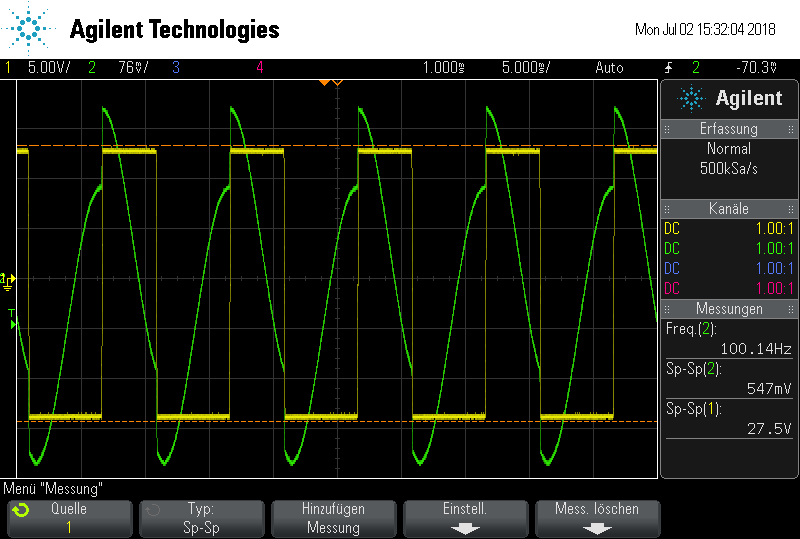
\includegraphics[height=0.3\textheight]{data/scope_268.png}
  %   \caption{Aufnahmen des Oszilloskops.}
  %   \label{fig:schmitt_osz}
  % \end{subfigure}
  % \begin{subfigure}{\textwidth}
    \centering
    \includegraphics[width=0.8\textwidth]{build/schmitt.pdf}
    \caption{Messwerte des Schmitt-Triggers mit markierter Schwelle der Sinuseingangsspannung.}
    \label{fig:schmitt_plot}
  % \end{subfigure}
  % \caption{Messwerte des Schmitt-Triggers.}
  \label{fig:schmitt}
\end{figure}

\subsection{Dreieckgenerator}
Ein Dreieckgenerator wird mit den Bauteilen
$C = \SI{20.8}{\nano\farad}$,
$R_1 = \SI{0.1}{\kilo\ohm}$,
$R_\text{P} = \SI{1}{\kilo\ohm}$,
$R = \SI{30.2}{\kilo\ohm}$
gebaut.
Es wird eine Betriebsspannung von $U_B = \SI{14.7}{\volt}$ angelegt.
In Abbildung~\ref{fig:dreieck_generator} wird ein Oszilloskopbild
der Ausgangsspannung des Dreieckgenerators dargestellt.
\begin{figure}[ht]
  \centering
  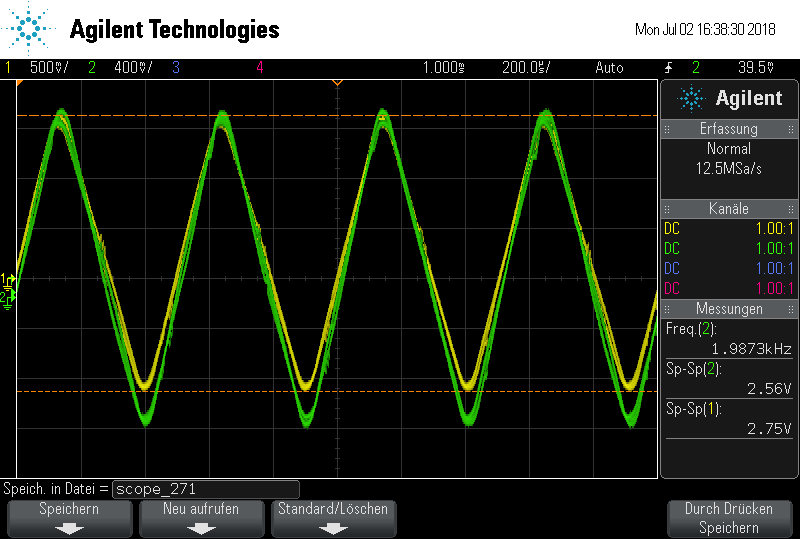
\includegraphics[height=0.3\textheight]{data/scope_271.png}
  \caption{Oszilloskopaufnahme des Dreieckgenerators.}
  \label{fig:dreieck_generator}
\end{figure}

Die Frequenz und Amplitude der Dreieckspannung werden am Oszilloskop abgelesen.
Die Theoriewerte werden aus Gleichung~\eqref{eq:schmitt} (Schmitt-Triggerpunkt, außerdem gelbe Linie in Abbildung~\ref{fig:dreieck_generator})
und Gleichung~\eqref{eq:integrator} berechnet:
\begin{align*}
  U_A &= \frac{-1}{RC} \int_{t_1}^{t_2} U_1(t) \text{d}t \\
  \intertext{mit $U_1(t) = \pm U_B$ die Ausgangsspannung des Schmitt-Triggers,}
  &= \frac{-1}{RC} U_B \left(t_2 - t_1\right).
  \intertext{Ab hier ist $\Delta t \coloneqq \left(t_2 - t_1\right)$ eine halbe Periode: $\Delta
  t = \sfrac{T}{2}$.
  Sei
  $U_A(t_2) = \sfrac{R_1}{R_P} U_B$
  und
  $U_A(t_1) = -\sfrac{R_1}{R_P} U_B$, so ist
  }
  -2 \frac{R_1}{R_P} U_B &= \frac{-1}{RC} U_B \Delta t
  \intertext{und daher}
  T = 2 \Delta t &= 4 \frac{R_1 RC}{R_P}.
\end{align*}

Die Amplitude ist
\begin{align*}
  A_\text{theo} &= U_B \frac{R_1}{R_P} = \SI{1.47}{\volt} \\
  A_\text{exp} &= \SI{1.28}{\volt} \\
  \Rightarrow \Delta A &= \SI{13}{\percent}.
\end{align*}

% Hierfür wird Gleichung~\eqref{eq:integrator_before} integriert, sodass für die Integrationsgrenzen $U(t_1) = \SI{0}{\volt}$ und $U(t_2) = U_S$ gilt, mit der Spannung beim Umschalten des Schmitt-Triggers $U_S$.
Die Frequenz der generierten Dreieckspannung wird am Oszilloskop abgelesen.
Es sind
\begin{align*}
  \nu_\text{theo} &= \frac{1}{T} = \SI{3.98}{\kilo\hertz} \\
  \nu_\text{exp}  &= \SI{1.99}{\kilo\hertz} \\
  \Rightarrow \Delta \nu &= \SI{50}{\percent}.
\end{align*}

\subsection{Ged\"ampfte Schwingung}
% =================================

\begin{figure}[ht]
  \centering
  \begin{subfigure}{\textwidth}
    \centering
    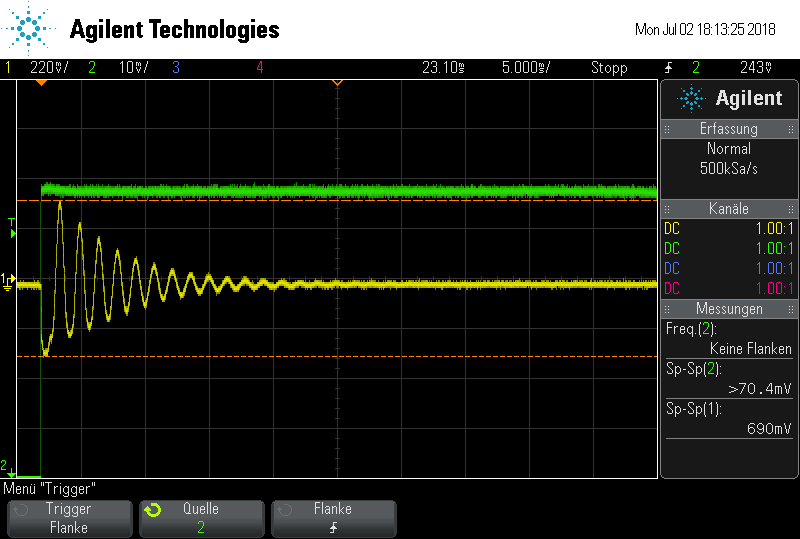
\includegraphics[height=0.3\textheight]{data/scope_275.png}
    \caption{Aufnahme des Oszilloskops.}%
    \label{fig:gedaempft_oszilloskop}
  \end{subfigure}
  \begin{subfigure}{\textwidth}
    \centering
    \includegraphics[width=0.8\textwidth]{build/gedaempfte_schwingung.pdf}
    \caption{Oszilloskopdaten mit Fit.}%
    \label{fig:gedaempft_fit}
  \end{subfigure}
  \caption{Messwerte und Fit der gedämpften Schwingung.}%
  \label{fig:gedaempft}
\end{figure}

Die Betriebsspannung wird auf $U_B = \pm \SI{1.95}{\volt}$ gestellt.
Die gedämpfte Schwingung ist in Abbildung~\ref{fig:gedaempft} dargestellt.
Es wird ein Fit der Form
\begin{equation}
  % U = \log{\left(x\right)} \cdot m + b
U = U_0 \cdot \exp{\left(\frac{-t}{\tau}\right)} \cdot \sin{\left(t \cdot \omega  + \phi\right)} + b
\end{equation}
in einem logarithmischen Diagramm (vgl. Abbildung~\ref{fig:gedaempft_fit}) aufgetragen.
Die Parameter des Fits sind
\begin{align*}
  U_0 &= \SI{-0.463 \pm 0.005}{\volt} \\
  \omega &= \SI{4260 \pm 3}{\per\second} \\
  \tau &= \SI{4.7 \pm 0.12}{\milli\second} \\
  b &= \SI{-0.023 \pm 0.004}{\volt} \\
  \phi &= \SI{-8.075 \pm 0.01}{\radian}.
\end{align*}
 Nach Gleichung~\eqref{eq:T_theo} und~\eqref{eq:tau_theo} ergeben sich mit
\begin{align*}
  R &= \SI{10}{\kilo\ohm} \\
  C &= \SI{20.8}{\nano\farad},
\end{align*}
die Theoriewerte und relativen Abweichungen der Fitparameter
\begin{align*}
  \omega_\text{theo} &= \frac{2\pi}{T} = \frac{1}{R C} = \SI{4800}{\per\second} \\
  \Rightarrow \Delta \omega &= \num{11}\% \\
  \tau_\text{theo} &= 20 RC = \SI{4.2}{\milli\second} \\
  \Rightarrow \Delta \tau &= \num{12}\%.
\end{align*}
